\documentclass[12pt]{article}
\usepackage{graphicx}
\usepackage{caption}
\usepackage{amsmath}
\usepackage{geometry}
\usepackage{float}
\usepackage{booktabs}
\usepackage{longtable}
\usepackage{setspace} % for spacing control
\usepackage{indentfirst}
\usepackage{titlesec}
\setstretch{1.0}       % single line spacing (default)
\setlength{\parskip}{0pt}   % no space between paragraphs
\setlength{\parindent}{0em} % set indentation amount

\geometry{margin=1in}
\setlength{\parskip}{0em}
\setlength{\parindent}{0pt}

\title{Assignment 2 \\ \large Computational Plasticity (SoSe25)}
\author{Bagus Alifah Hasyim \\ 108023246468}
\date{}

\begin{document}
\maketitle

\section*{Given Data}
\hspace*{2em}In this section, the parameters value for the material properties, 
that required by the author to calculate it based on the author's Immatrikulation Nummer, will be defined accordingly. To make
the calculation detailed and transparent, each parameter will be derived step by step. 

\begin{equation}
    a = 4, \text{   }\text{   } b = 6, \text{   }\text{   } c = 8
\end{equation}

\vspace{1em}
Parameter for 1st question:
\begin{itemize}
    \item $E = 200 + (10 \times a) = 200 + (10 \times 4 ) = 240 \;\text{GPa}$  
    
\end{itemize}

\vspace{1em}
Parameter for 2nd question:
\begin{itemize}
    \item $\sigma_y = 600 + (a \times 33) = 600 + (4 \times 33) = 600 + 132 = 732 \;\text{MPa}$
    \item $C_1 = 10000 + b \times 1666 = 10000 + 6 \times 1666 = 10000 + 9996 = 19996 \;\text{MPa}$
    \item $\gamma_1 = 200 + (10 \times c) = 200 + (10 \times 8) = 280 \;\text{MPa}$
    \item $C_2 = 3000 + (a \times 166) = 3000 + (4 \times 166) = 3000 + 664 = 3664 \;\text{MPa}$
\end{itemize}

\vspace{1em}
Parameter for 3rd question:
\begin{itemize}
    \item $\sigma_{ya} = 300 + (10 \times b ) = 300 + (10 \times 6) = 300 + 60 = 360 \;\text{MPa}$
\end{itemize}

\section{Introduction}
\hspace*{2em}For this second assignment, mechanical response analysis will be conducted using a
simple squared geometry model with a circular inclusion in the center. Hence, the analysis will be 
divided into three tasks. The first task is mesh sensitivity analysis, where the main goal of this first 
task is to see the influence of variety of mesh sizes to the captured stress concentration generation along the defined line
from the edge of the circular hole until the opposite edge of the plate. Then there's 
come the second task, where the focus will be to investigate the isotropic and kinematic hardening 
effect to its mechanical response. The last task is a subroutine implementation, where the objective
is to point out the difference between the standard and UMAT results. Extracting some other information will be done 
as well in the third task. 

\hspace*{2em}In this following section, each question will systematically will be addressed in the assignment,
providing detailed explanations, derivations, and relevant figures or tables to support the
analysis. All calculations and results are based on the provided data and the author’s
unique identification number. Numerical analysis will be performed using Abaqus CAE
with an appropriate boundary condition and settings. 


\section{Set up of the Model}
\hspace*{2em}For the model setup, 2D planar-deformable shell-model will be used for the plate with the specified geometry, boundary condition, material properties, and mesh.  
\subsection{Geometry and Boundary Conditions}

\begin{figure}[H]
    \centering
    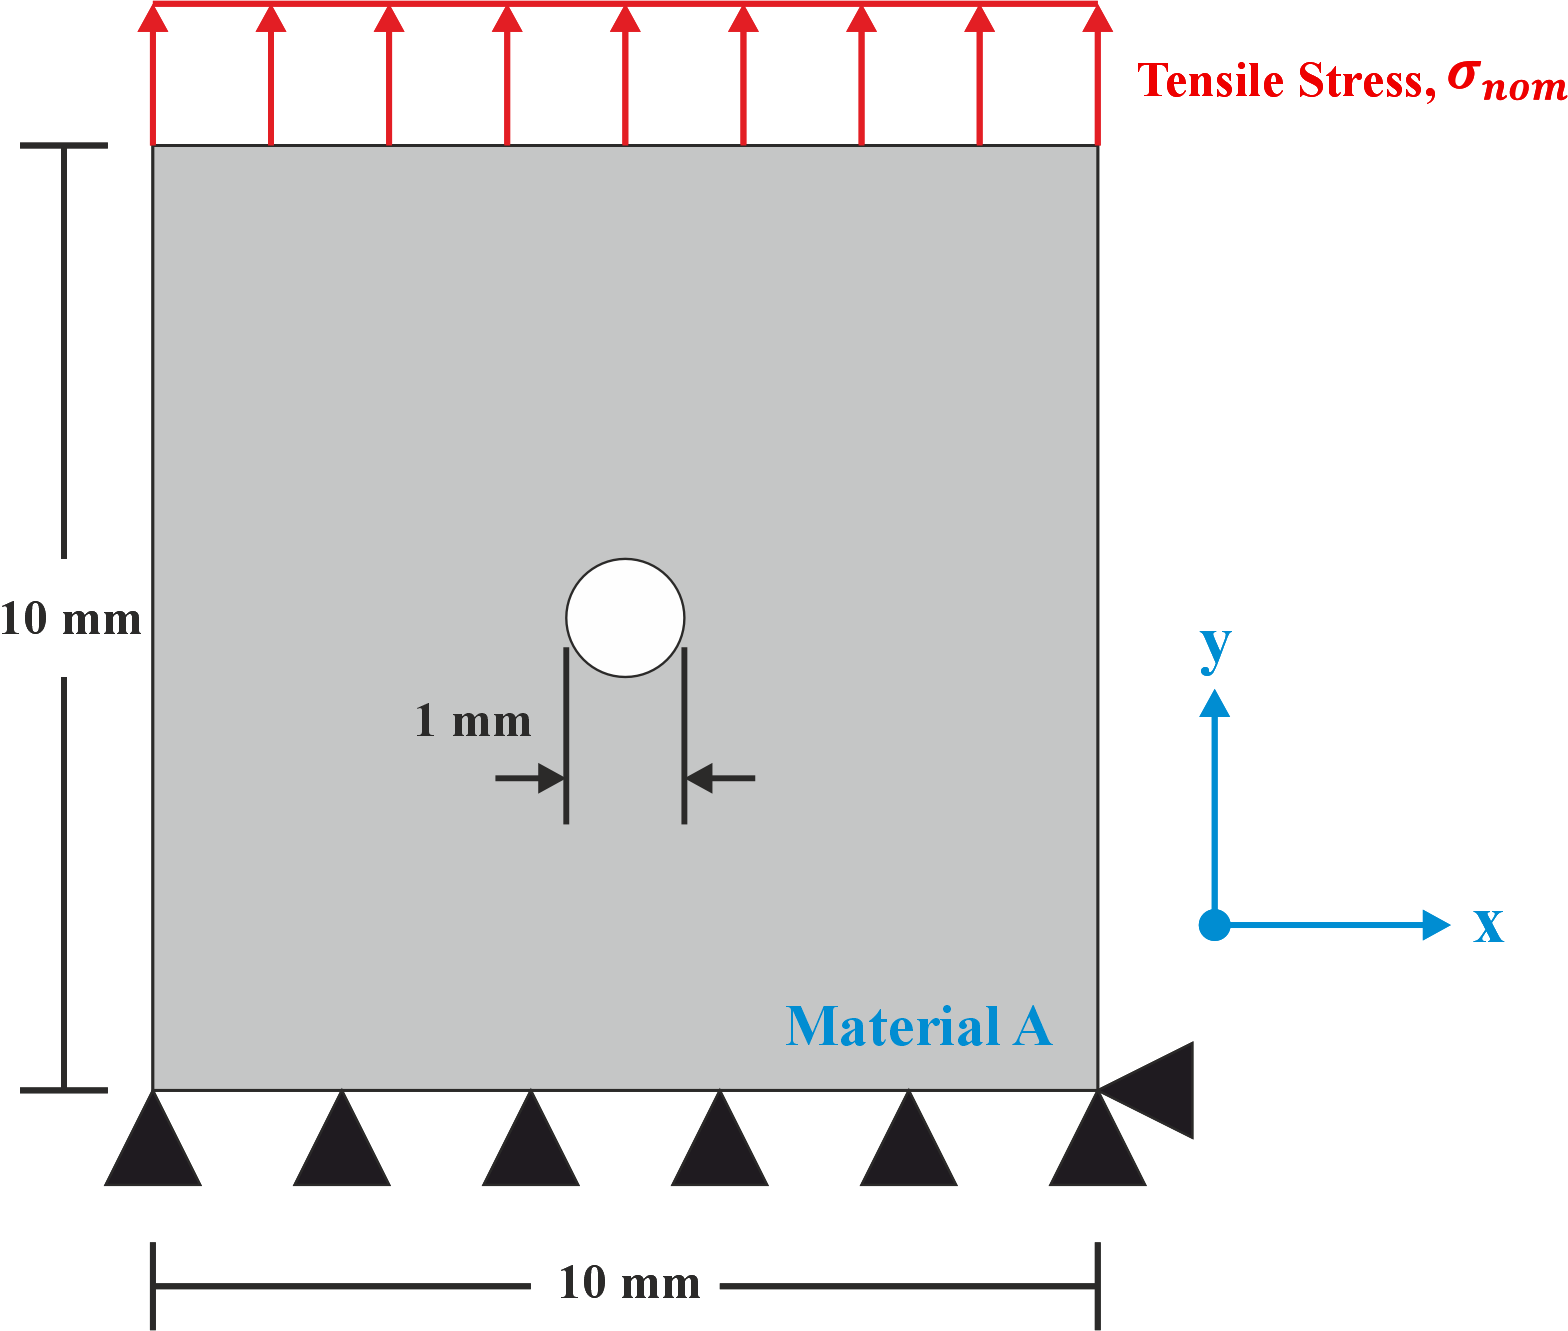
\includegraphics[width=0.6\textwidth]{images/GEO_Base.png}
    \caption{Baseline plate geometry with defined material A with thickness $t = 1 \;\text{mm}$. Two boundary conditions are applied, which are the 
        fixed support restriction in y direction on the bottom line of the plate, fixed support point on the bottom right point restriction to 
        x direction, and stress constant distribution along the top plate line with value of $\sigma_{nominal} = 1 \;\text{MPa}$}
\end{figure}

\subsection{Material Properties}
\hspace*{2em}The material properties used in the analysis are provided in the task definition. However, 
some parameters must be manually calculated based on the author's Immatrikulation Nummer in the very first section.

\begin{table}[H]
    \centering
    \caption{Elastic properties for Q1.}
    \label{tab:materialQ1-properties}
    \begin{tabular}{ll}
        \toprule
        E (GPa) & $\nu$ (Poisson's Ratio) \\
        \midrule
        \multicolumn{1}{c}{240} & \multicolumn{1}{c}{0.3} \\
        \bottomrule
    \end{tabular}
\end{table}

\begin{table}[H]
    \centering
    \caption{Material parameters (combined hardening law) for Q2.}
    \label{tab:materialQ2-properties}
    \begin{tabular}{lccccccc}
        \toprule
        $\sigma_y$ (MPa) & $C_1$ (MPa) & $\gamma_1$ & $C_2$ (MPa) & $\gamma_2$ & Q-Infinity & Hardening Param $b$ \\
        \midrule
        732 & 19996 & 280 & 3664 & 0 & 440 & 20 \\
        \bottomrule
    \end{tabular}
\end{table}

\begin{table}[H]
    \centering
    \caption{Plastic properties for Q3}
    \label{tab:materialQ3-properties}
    \begin{tabular}{lll}
        \toprule
            \centering $\sigma_{ya}$ (MPa) & $\sigma_f$ (MPa) & $\epsilon_{p}^f$  \\
            \midrule
            \centering 360 & 550 & 0.4  \\
            \bottomrule
    \end{tabular}
\end{table}

\subsection{Meshing}

\hspace{2em}The baseplate with circular hole is mesh using a structured mesh, hence 
the partitioning is well-defined to ensure a good mesh quality. As requested by the task, 
the baseplate is partitioned using the general formatting guidelines. However, the author 
have the freedom to adjust the partitioned size. Therefore, for this assignment the dimensioning
of the mesh partition follows the provided Figure~\ref{fig:MeshPartitioning}. 

\hspace{2em} After the plate partitioning, specifically for task 1, the baseplate will be mesh
using 8 variations in the mesh size, where it is based on the global and local mesh size. 
The global mesh size is defined as the mesh size for the entire plate, 
while the local mesh size is defined as the mesh size around the circular hole (hence is the
area inside the small square partition). This method is done in order to capture the stress
concentration effects on the area near the hole accurately while maintaining a low computational
effort since the mesh size is not fine for the whole plate.

\hspace{2em}In order to know the mesh influence on the results, a mesh sensitivity
analysis is performed. This analysis involves systematically varying the mesh sizes and observing the effects on the simulation results, 
particularly the stress distribution around the circular hole. Therefore, mesh variation in
table~\ref{tab:mesh-sizes} is used for this study. 


\begin{figure}[H]
    \centering
    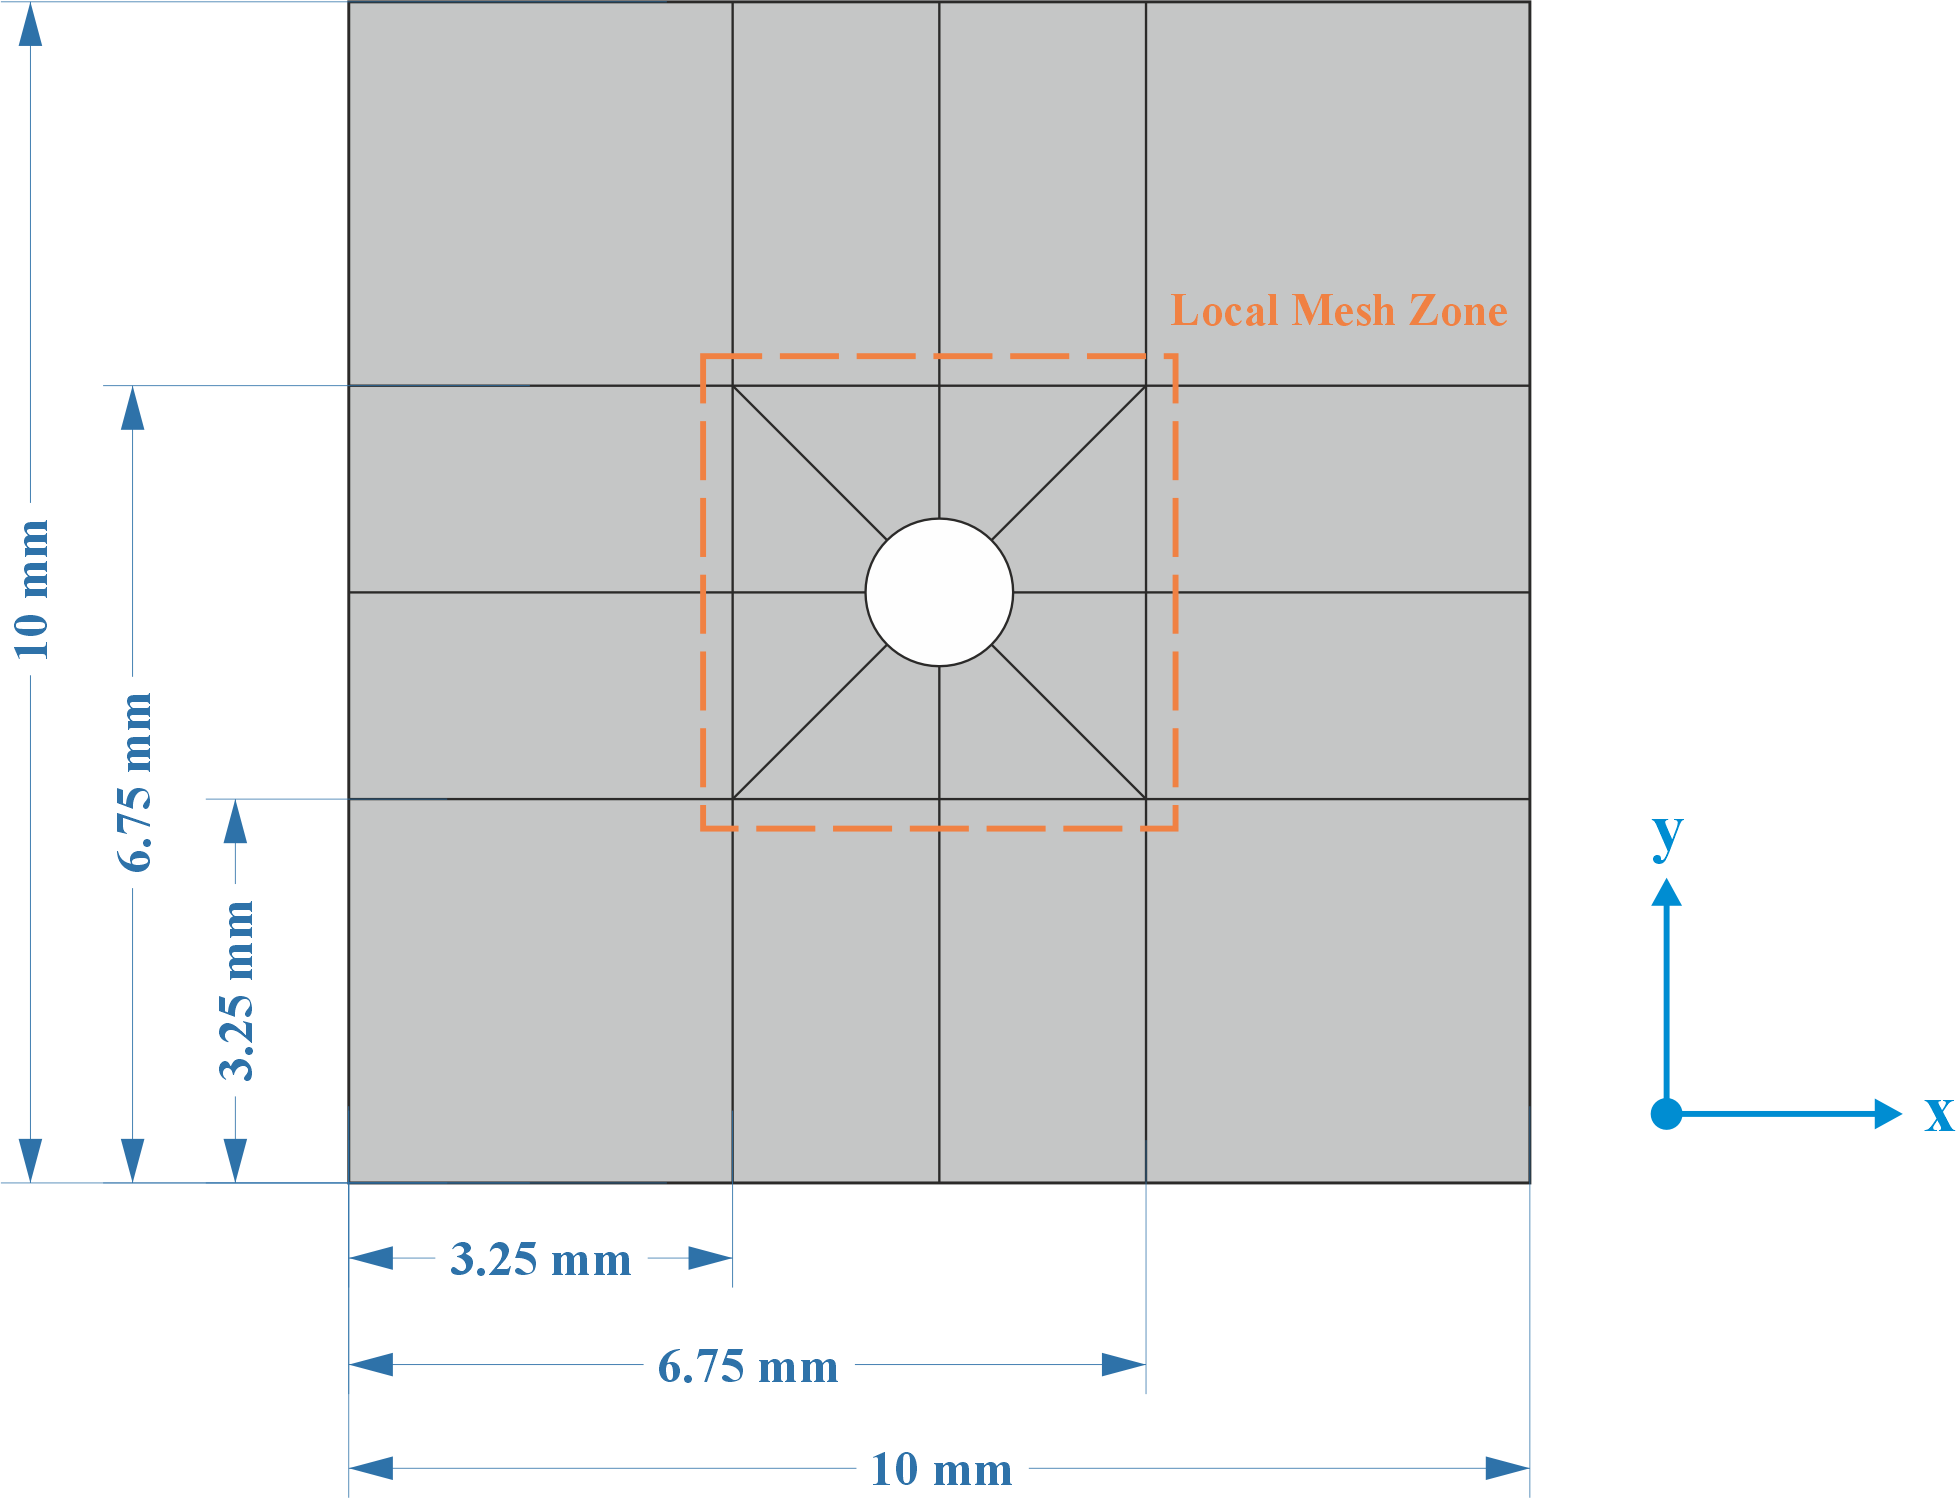
\includegraphics[width=0.9\textwidth]{images/MESH_Base.png}
    \caption{Partitioning guideline in order to create a structured mesh for the plate with
    circular hole. The whole mesh variations use CPS4, which is a 4-node bilinear plane stress quadrilateral element, 
    also using quad-structured mesh control feature for the whole region to retain structured mesh
    and avoid extreme-distorted element.}
\label{fig:MeshPartitioning}
\end{figure}

\begin{table}[H]
    \centering
    \caption{Mesh size variations used for mesh sensitivity analysis.}
    \label{tab:mesh-sizes}
    \begin{tabular}{ccc}
        \toprule
        Mesh Number & Global Mesh Size (mm) & Local Mesh Size (mm) \\
        \midrule
        1 & 1 & 1 \\
        2 & 1 & 0.6 \\
        3 & 0.8 & 0.4 \\
        4 & 0.6 & 0.3 \\
        5 & 0.4 & 0.2 \\
        6 & 0.3 & 0.1 \\
        7 & 0.2 & 0.05 \\
        8 & 0.1 & 0.02 \\
        \bottomrule
    \end{tabular}
\end{table}

\noindent
\textbf{Table Description:} This table summarizes the eight mesh configurations used in the mesh sensitivity analysis. Each mesh is defined by its global mesh size (applied to the entire plate) and a finer local mesh size (applied around the circular hole) to accurately capture stress concentrations while optimizing computational efficiency.

\begin{figure}[H]
    \centering
    \begin{minipage}{0.24\textwidth}
        \centering
        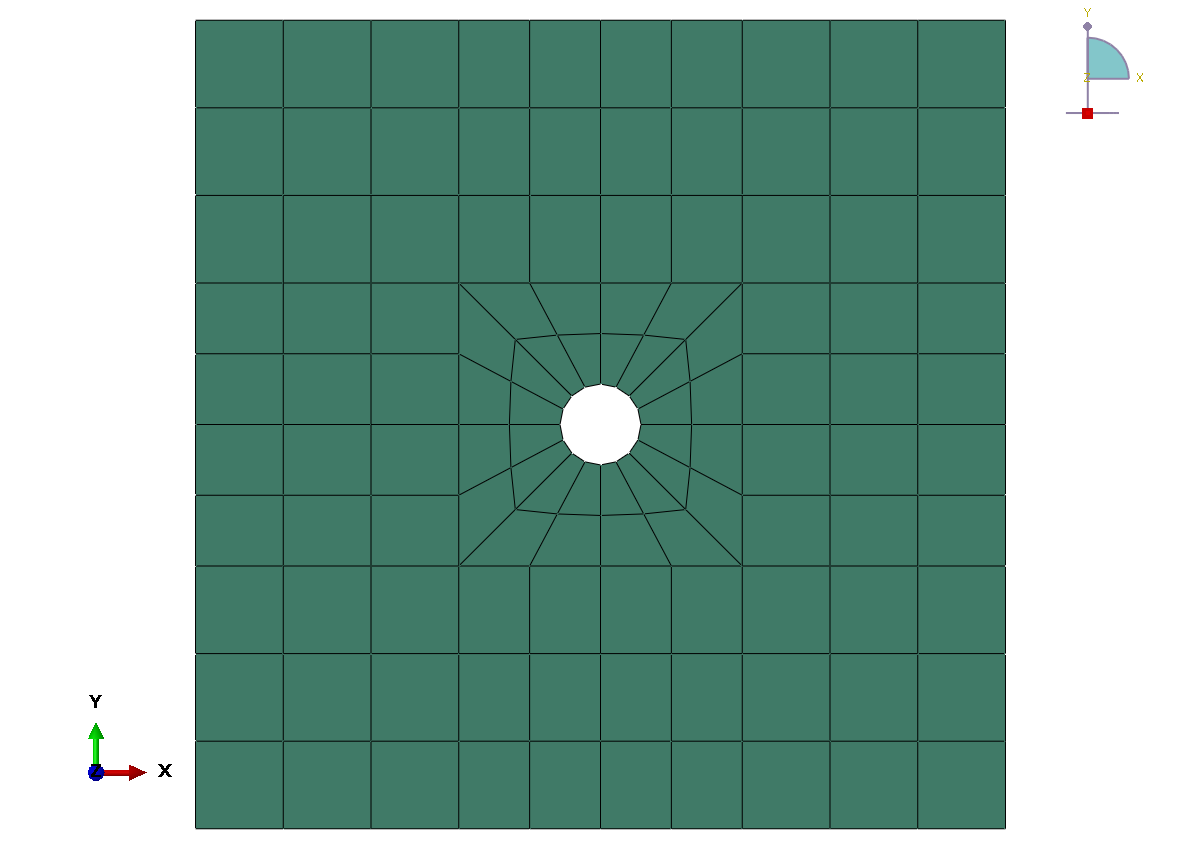
\includegraphics[width=\textwidth]{images/Mesh1.png}
        \caption*{116 elements.}
    \end{minipage}
    \begin{minipage}{0.24\textwidth}
        \centering
        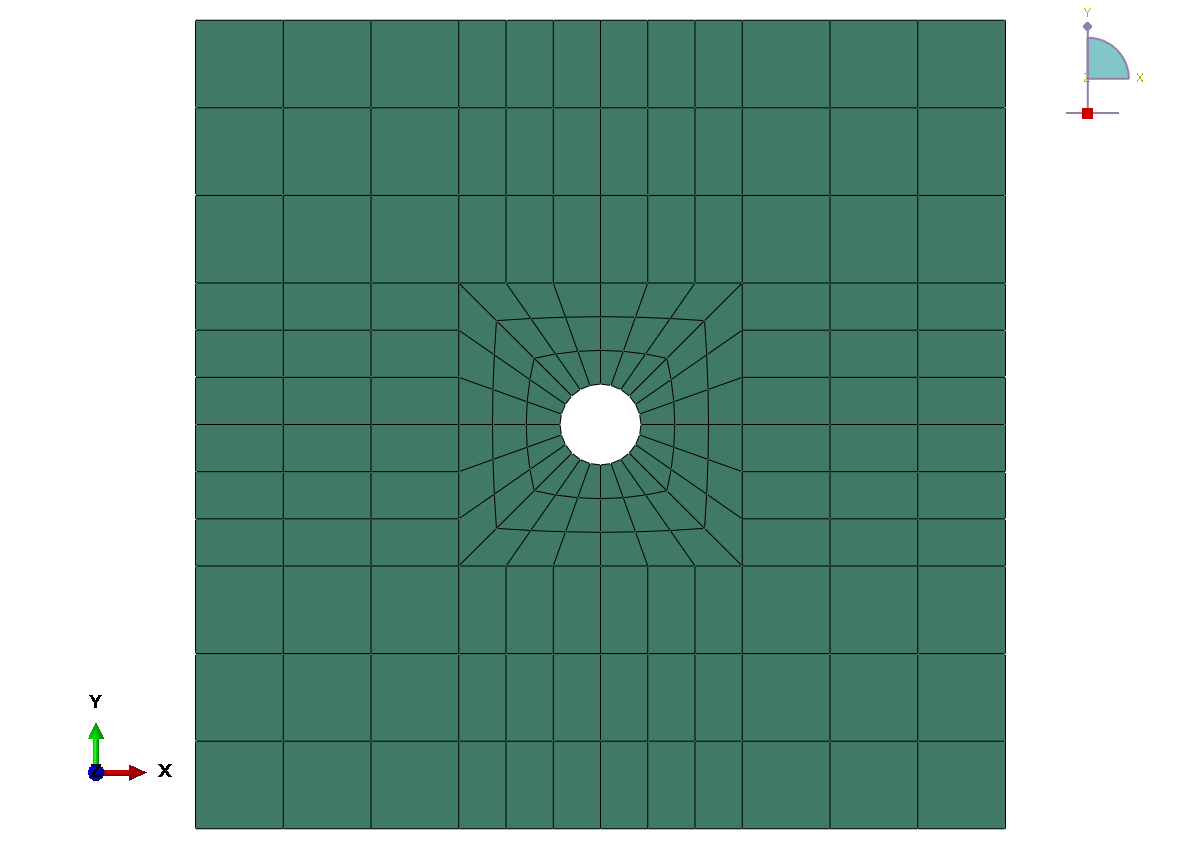
\includegraphics[width=\textwidth]{images/Mesh2.png}
        \caption*{180 elements.}
    \end{minipage}
    \begin{minipage}{0.24\textwidth}
        \centering
        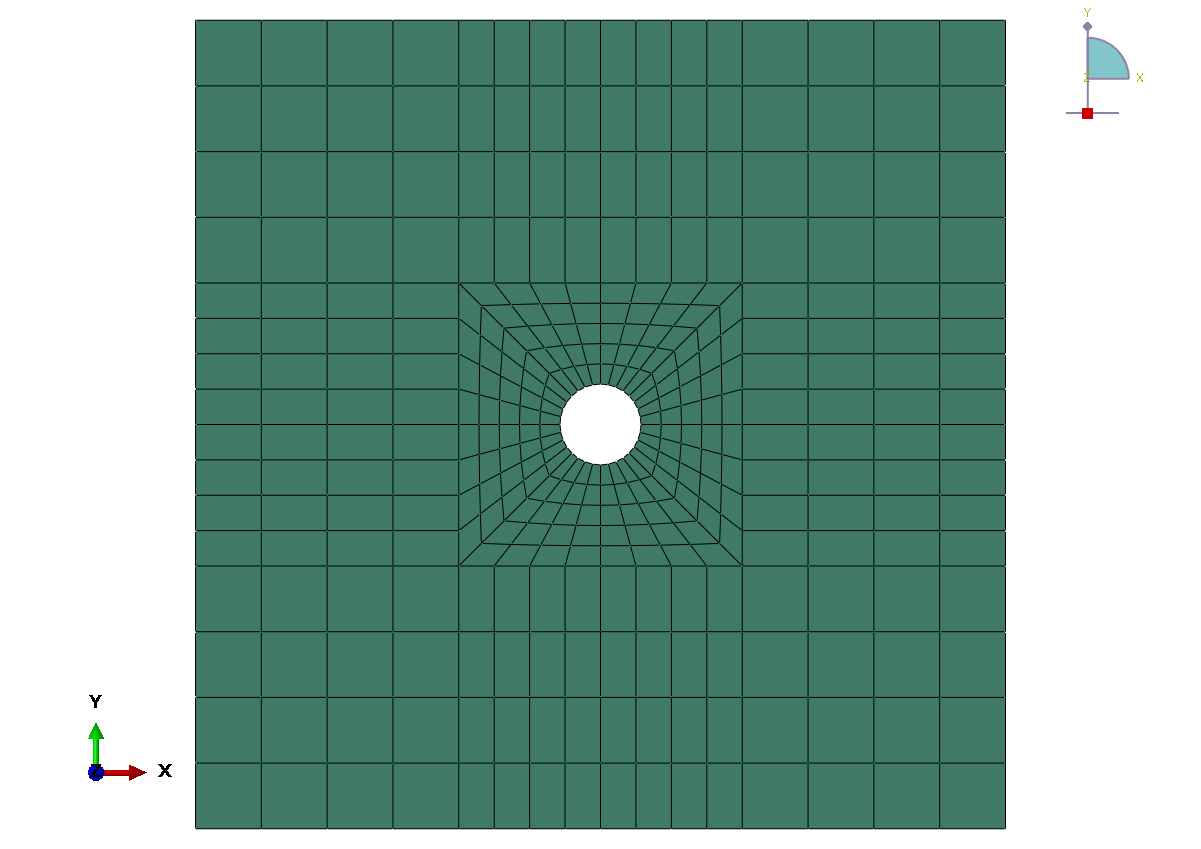
\includegraphics[width=\textwidth]{images/Mesh3.png}
        \caption*{352 elements.}
    \end{minipage}
    \begin{minipage}{0.24\textwidth}
        \centering
        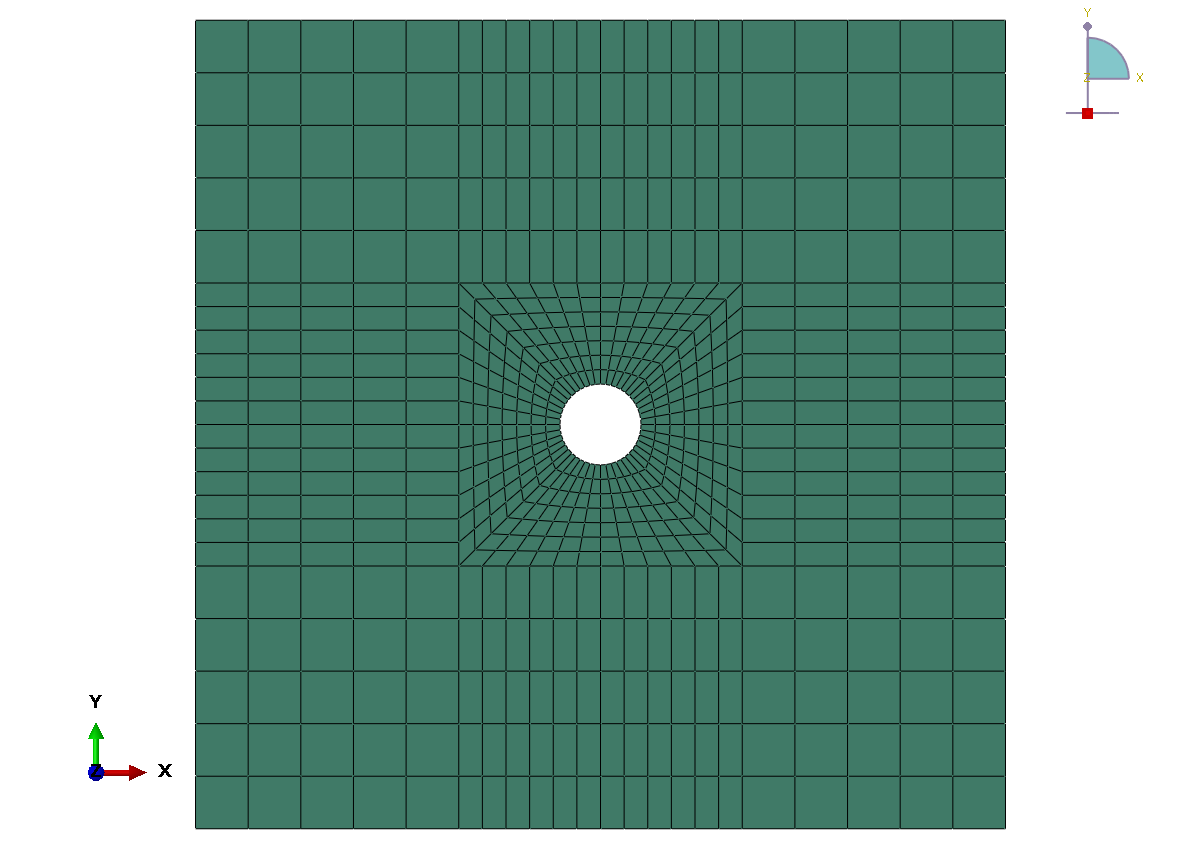
\includegraphics[width=\textwidth]{images/Mesh4.png}
        \caption*{676 elements.}
    \end{minipage}
\end{figure}

\begin{figure}[H]
    \centering
    \begin{minipage}{0.24\textwidth}
        \centering
        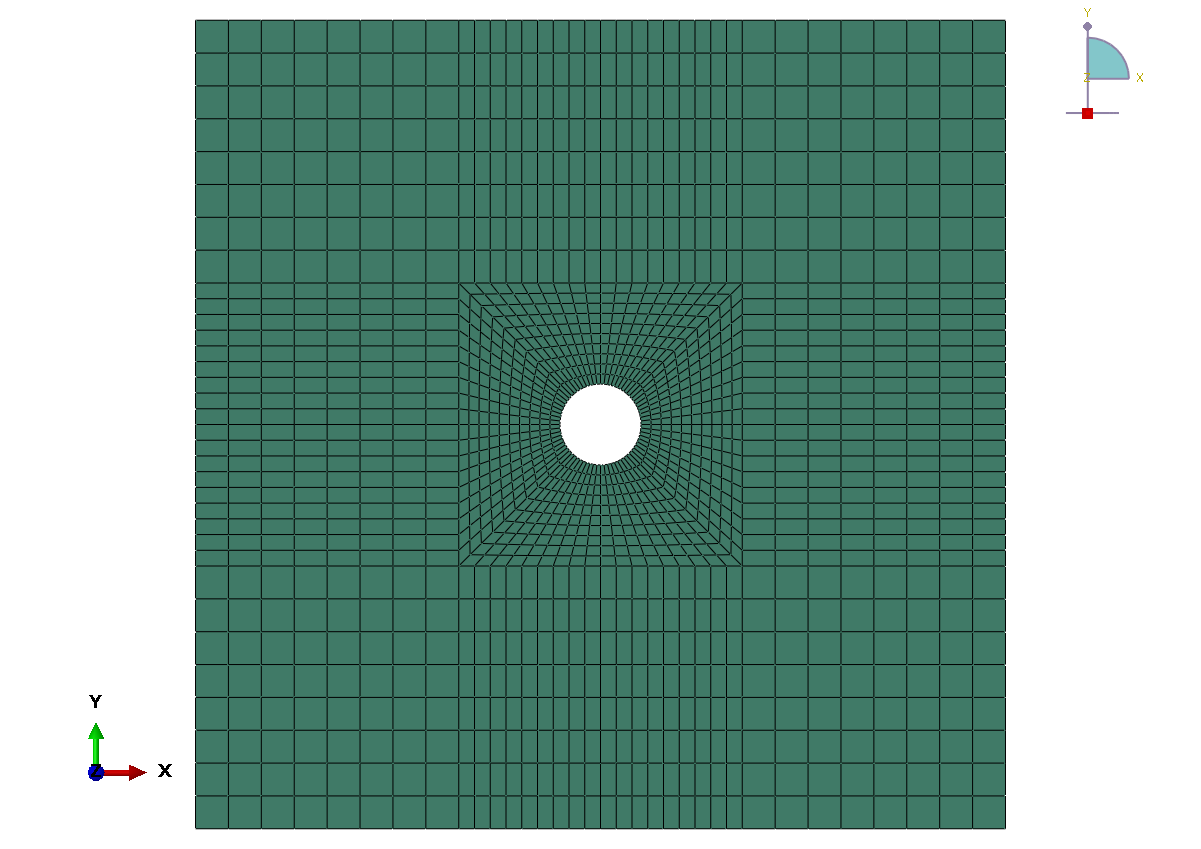
\includegraphics[width=\textwidth]{images/Mesh5.png}
        \caption*{1552 elements.}
    \end{minipage}
    \begin{minipage}{0.24\textwidth}
        \centering
        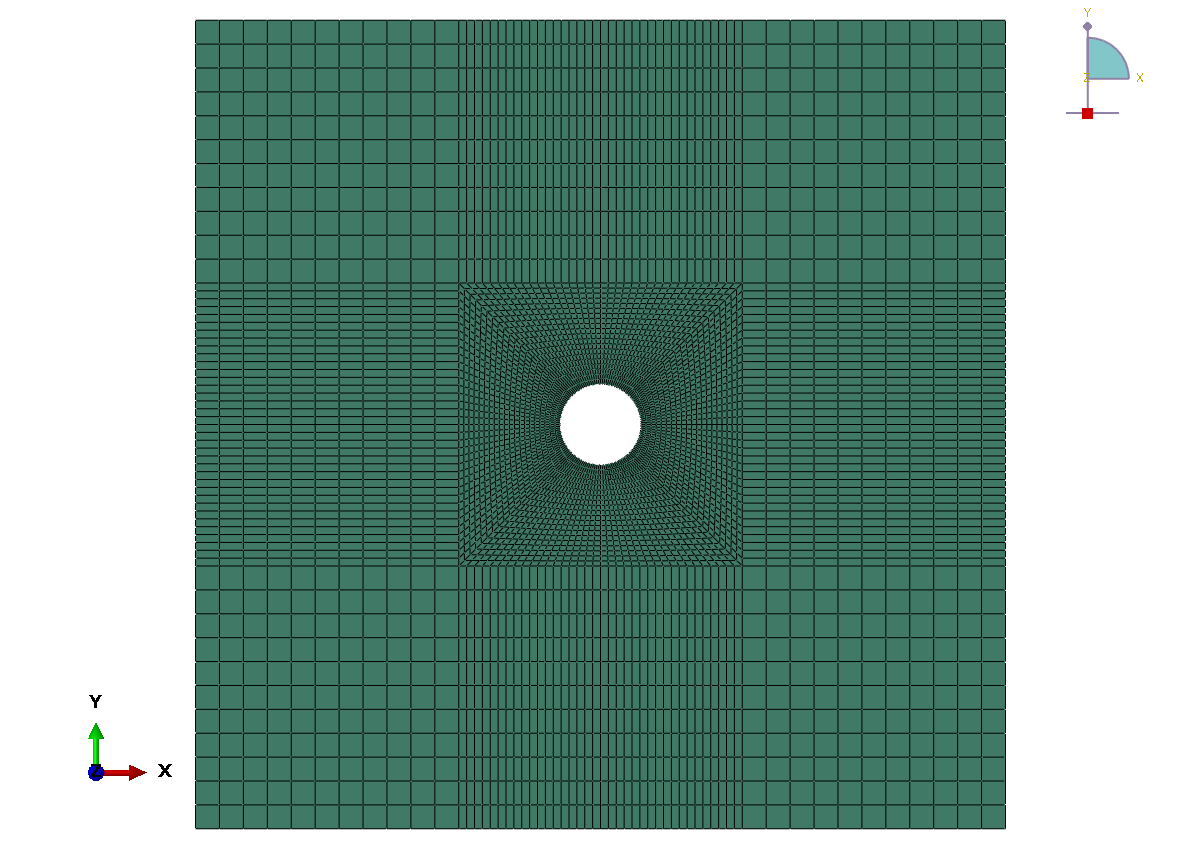
\includegraphics[width=\textwidth]{images/Mesh6.png}
        \caption*{4948 elements.}
    \end{minipage}
    \begin{minipage}{0.24\textwidth}
        \centering
        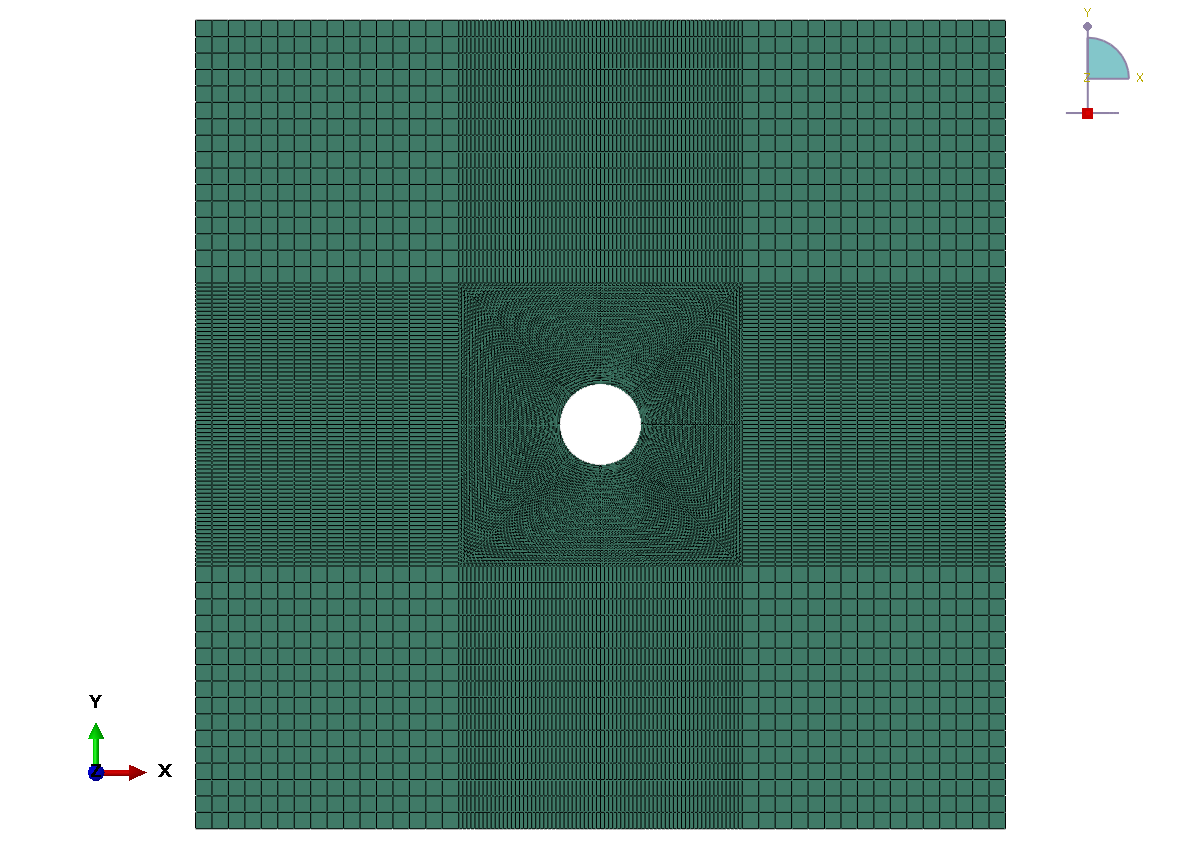
\includegraphics[width=\textwidth]{images/Mesh7.png}
        \caption*{16424 elements.}
    \end{minipage}
    \begin{minipage}{0.24\textwidth}
        \centering
        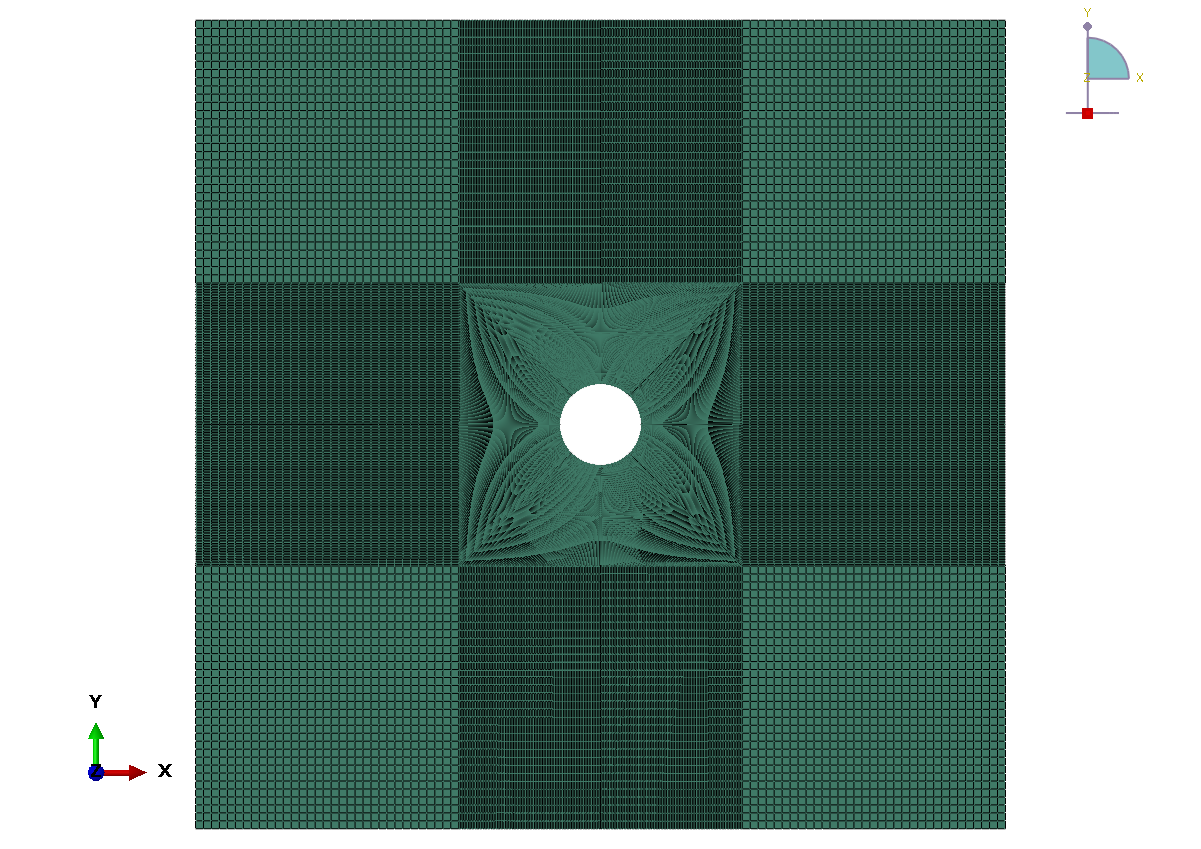
\includegraphics[width=\textwidth]{images/Mesh8.png}
        \caption*{97042 elements}
    \end{minipage}
\end{figure}
\section*{Results and Discussion}

\subsection*{Q1: Mesh Sensitivity Analysis of plate with circular hole}

\vspace{1em}
\textit{$\dots$ Create the model as shown in figure 1, using the face partitioning illustrated in figure 2, 
and apply the following assumptions: small deformations, plane stress conditions, 
and a homogeneous, isotropic, linear elastic material. For each mesh size specified in 
table 1, create a separate Job. Apply the local mesh size around the hole and use the 
global mesh size for the remaining regions of the plate.}

\vspace{1em}
\textit{$\dots$ For each mesh size, provide a figure exported directly from the 
Abaqus software (not a screenshot of the interface).}

\vspace{1em}
\textit{$\dots$ For each mesh size, provide a contour plot of the relevant stress component, 
with indicating the locations of both maximum and minimum stress values on the plot. 
Please ensure the contour plots are clearly presented, and the values are readable.}

\begin{figure}[H]
    \centering
    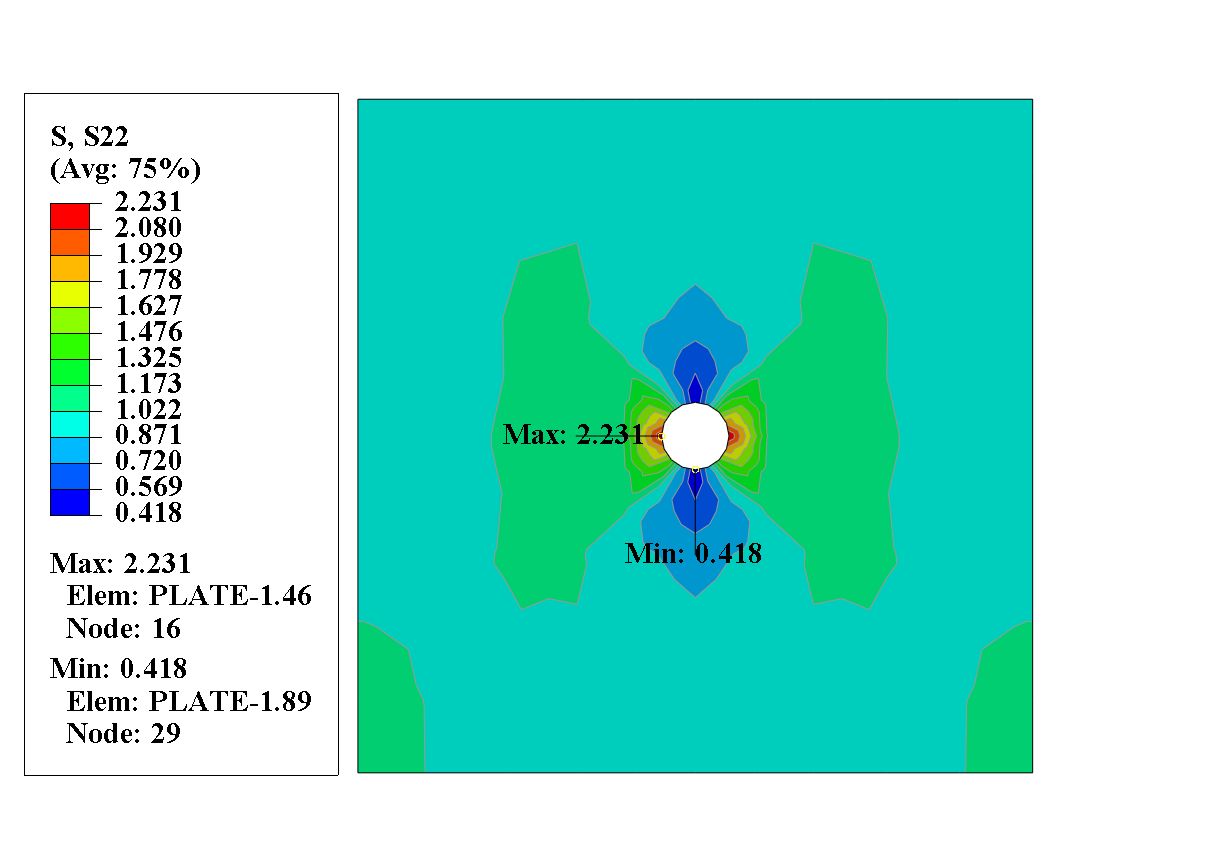
\includegraphics[width=0.48\textwidth]{images/S22_Mesh1.png}
    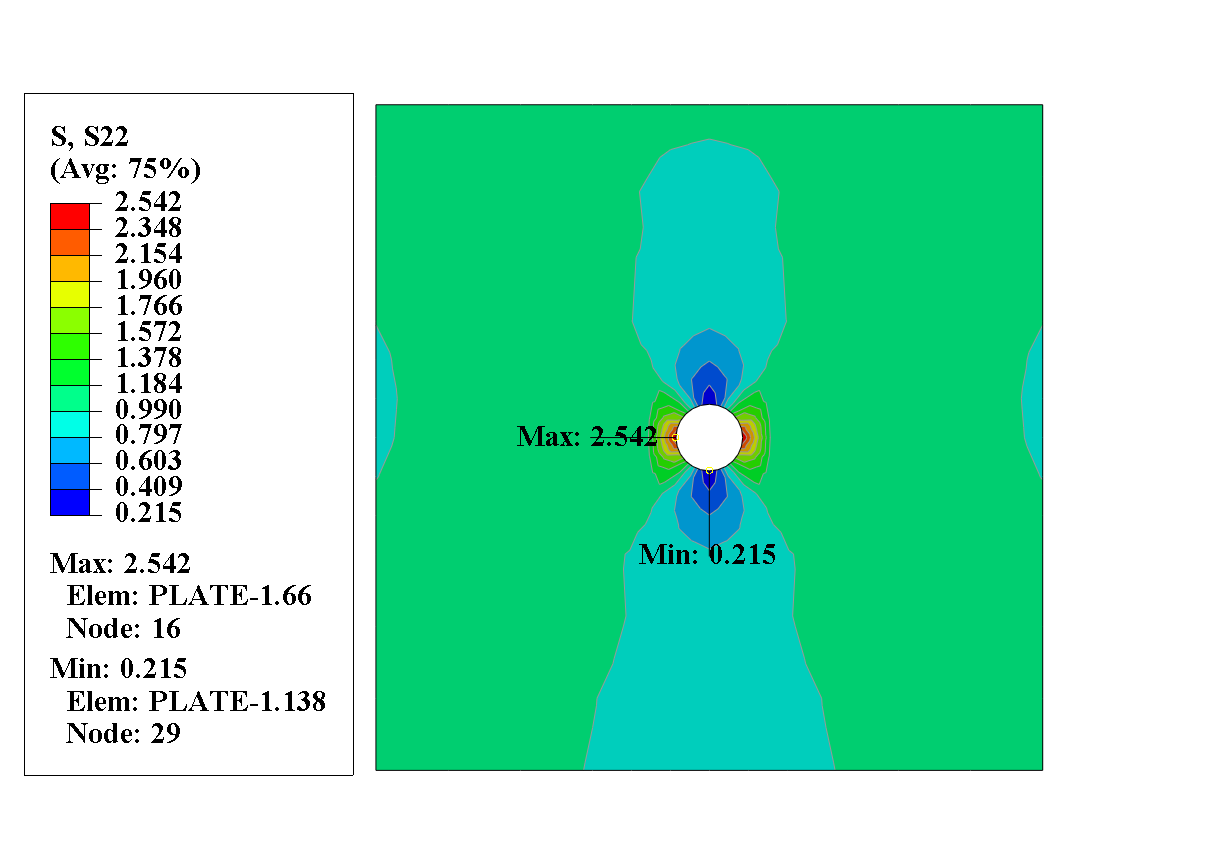
\includegraphics[width=0.48\textwidth]{images/S22_Mesh2.png}\\[-1.1em]
    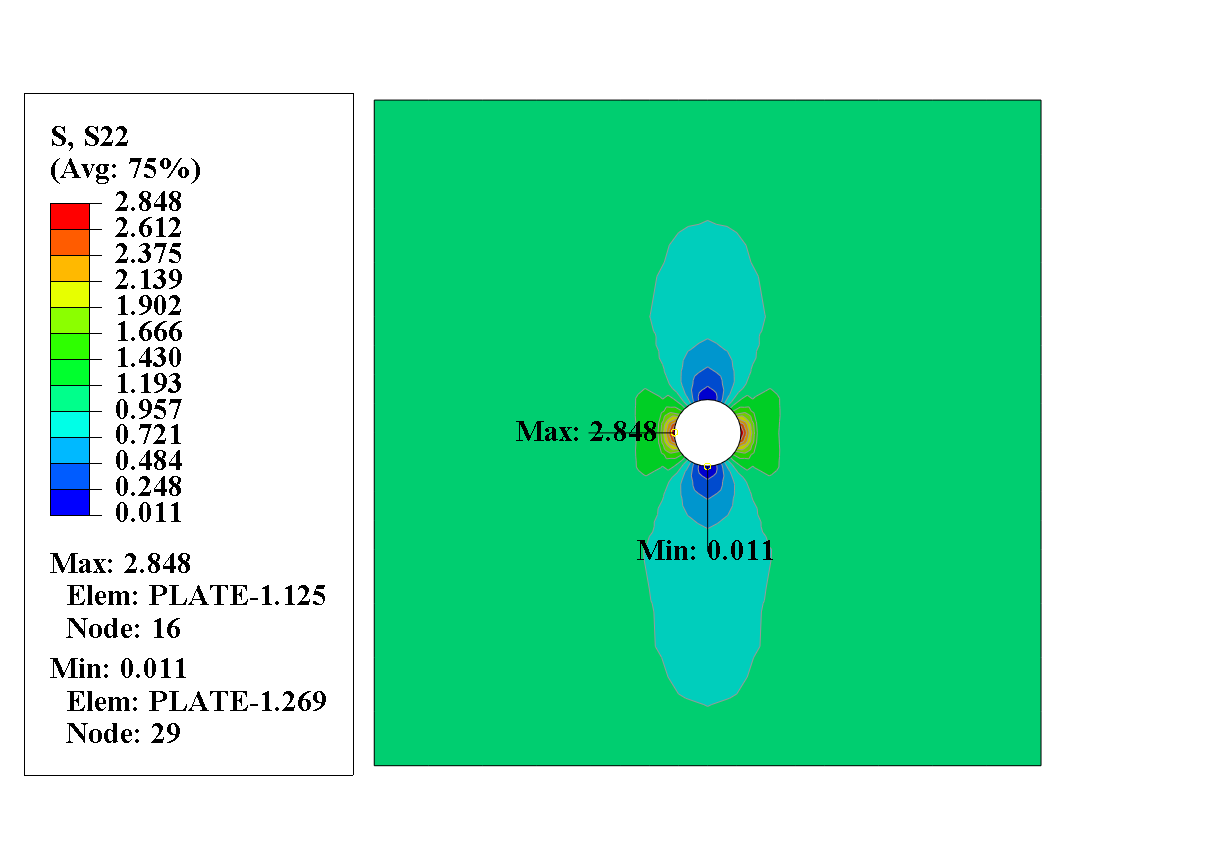
\includegraphics[width=0.48\textwidth]{images/S22_Mesh3.png}
    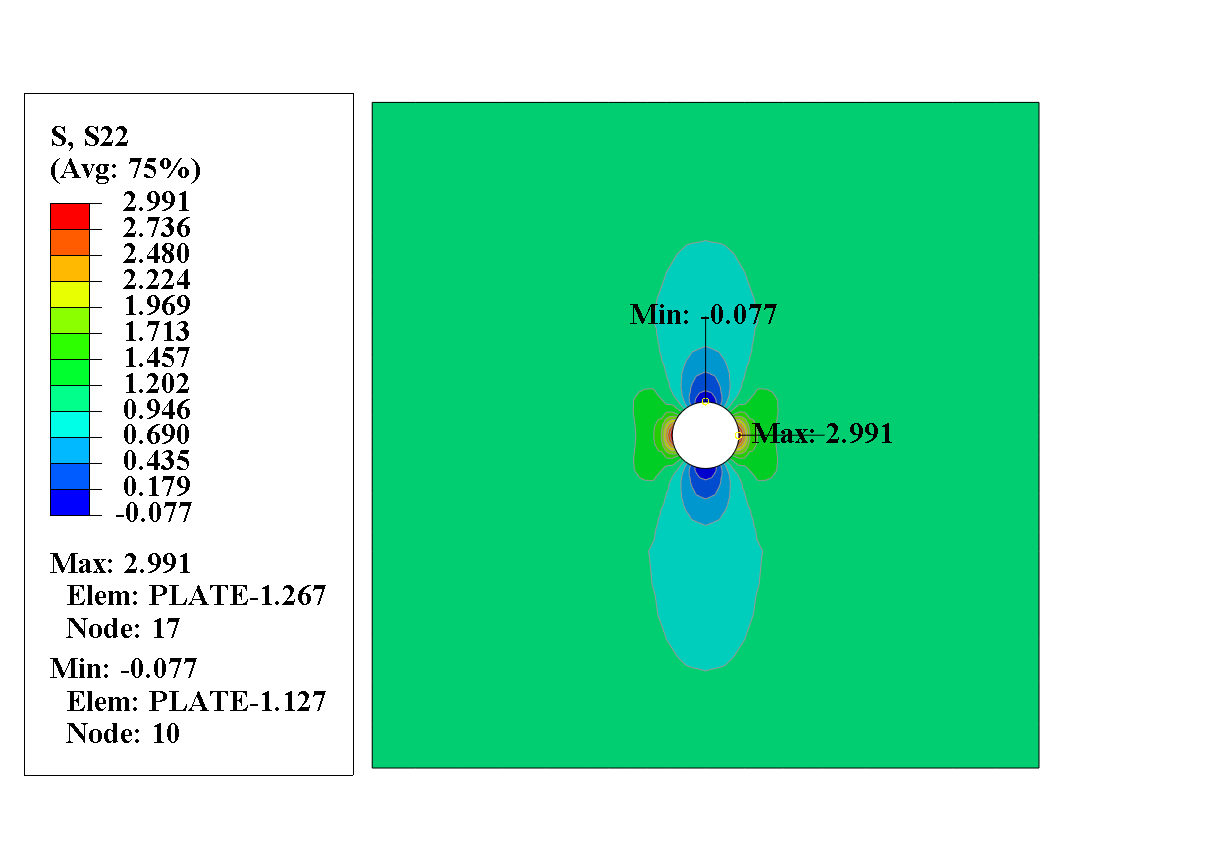
\includegraphics[width=0.48\textwidth]{images/S22_Mesh4.png}
    \caption{Contour plots of the $S_{22}$ stress component for Mesh 1, 2, 3, and 4 (from left to right, top to bottom). Maximum and minimum stress locations are indicated.}
    \end{figure}

    \begin{figure}[H]
    \centering
    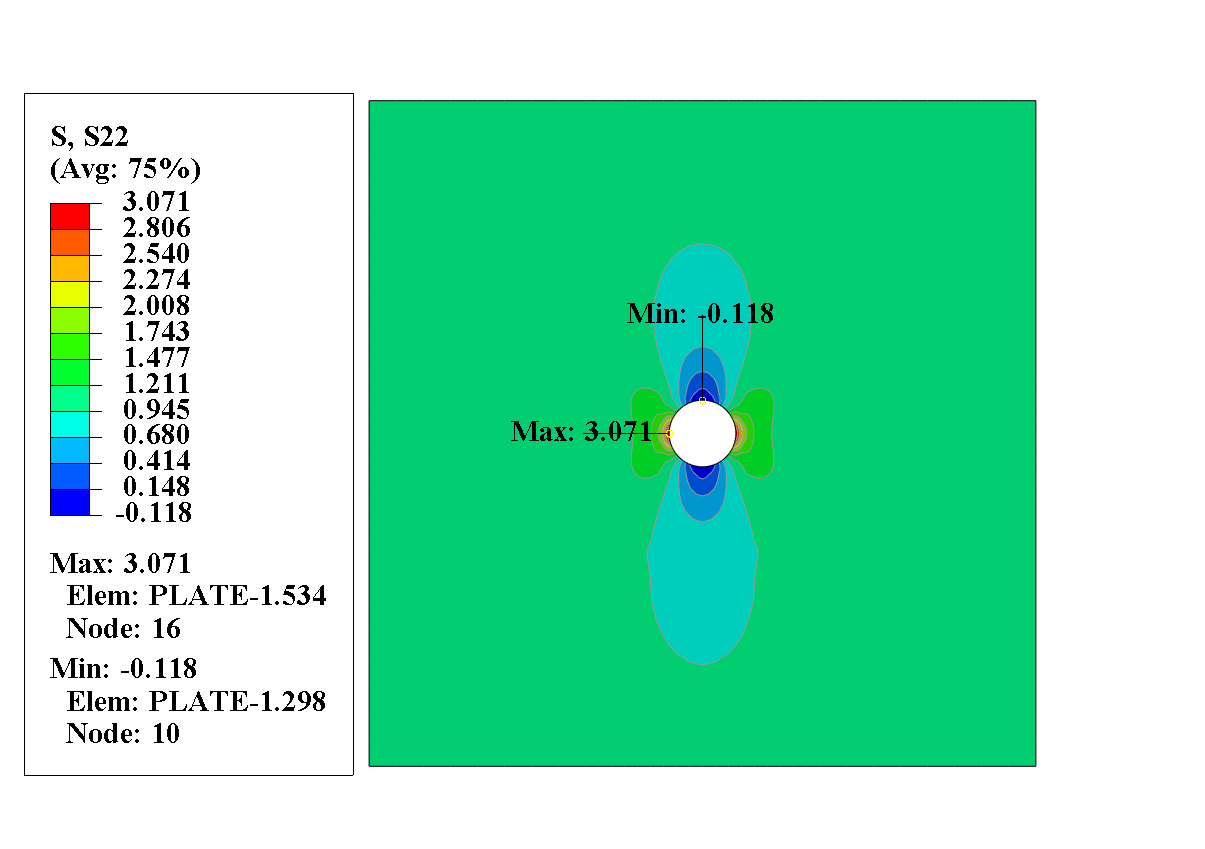
\includegraphics[width=0.48\textwidth]{images/S22_Mesh5.png}
    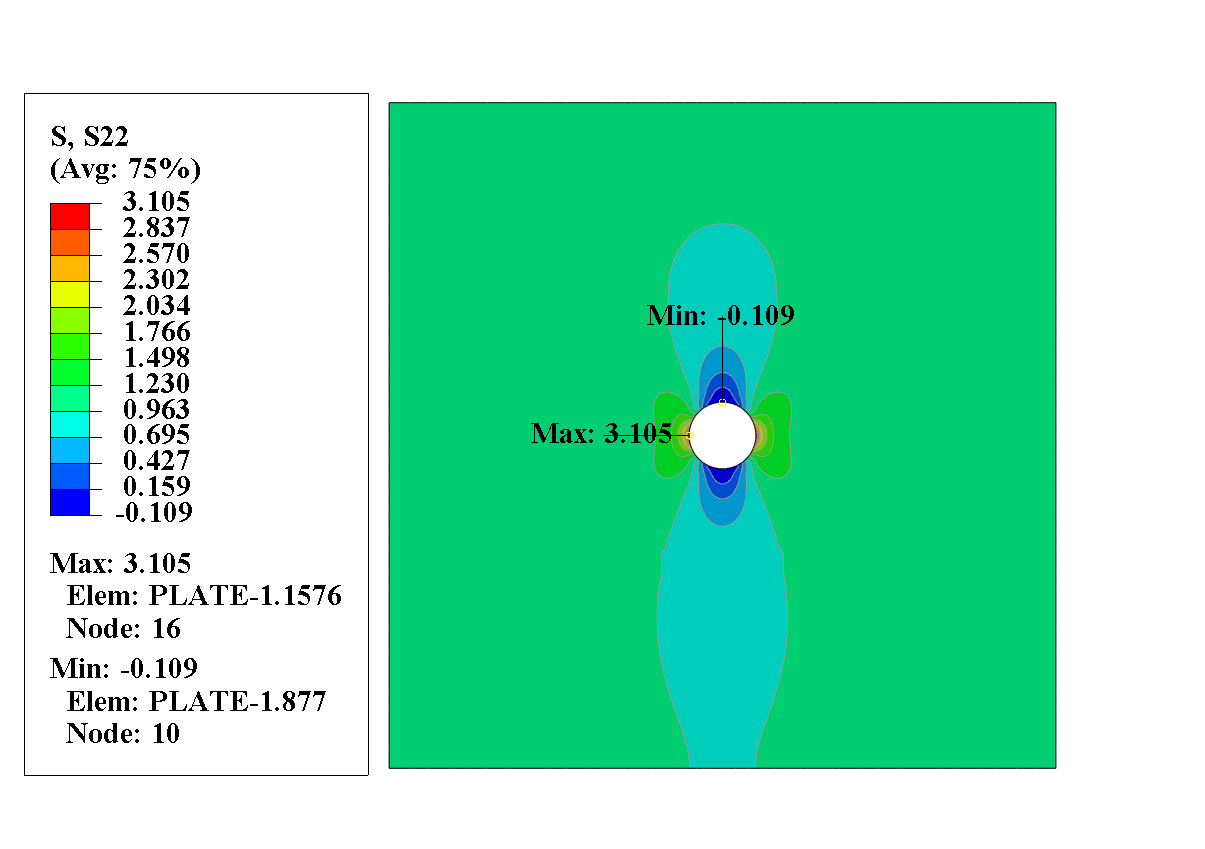
\includegraphics[width=0.48\textwidth]{images/S22_Mesh6.png}\\[-1.1em]
    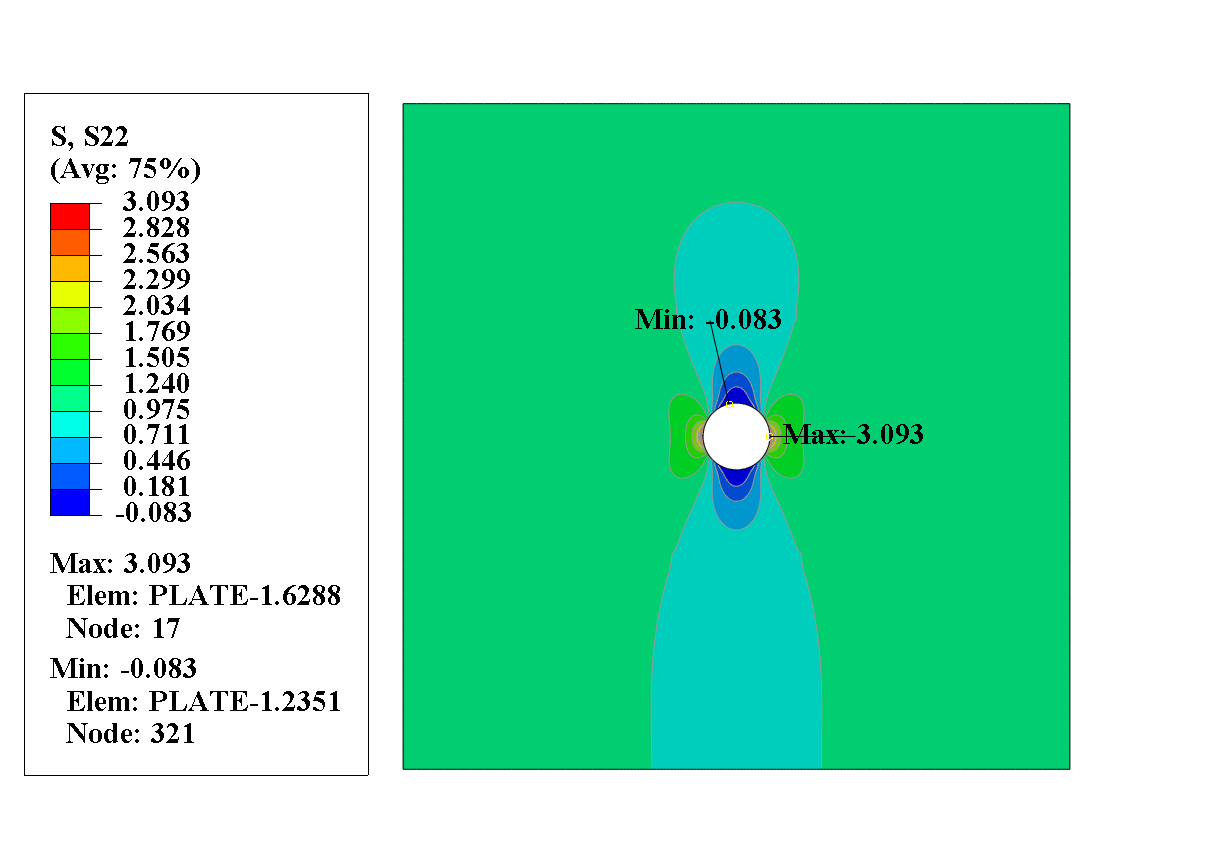
\includegraphics[width=0.48\textwidth]{images/S22_Mesh7.png}
    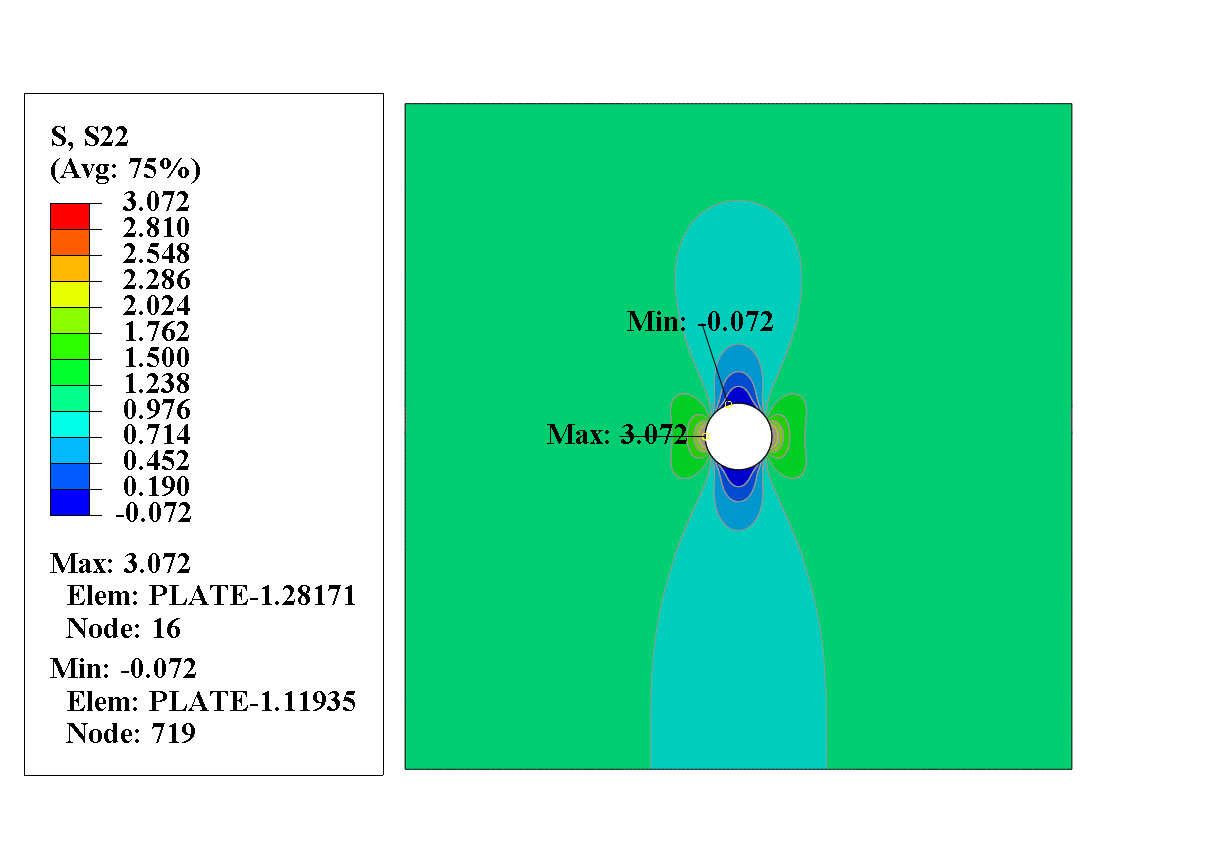
\includegraphics[width=0.48\textwidth]{images/S22_Mesh8.png}
    \caption{Contour plots of the $S_{22}$ stress component for Mesh 5, 6, 7, and 8 (from left to right, top to bottom). Maximum and minimum stress locations are indicated.}
    \end{figure}

\vspace{1em}
\textit{$\dots$ For each mesh size, calculate the stress concentration factor $K_t = \sigma_{max} / \sigma_{nom}$, 
You are required to provide two plots: the first plot should show eight curves 
(one for each mesh size), the relevant stress over the path. 
The second plot should display the mesh number against $K_t$. 
Based on the results, discuss and justify which mesh provides the most accurate and 
efficient representation of stress concentration, and explain why it should be chosen.}

\begin{figure}[H]
    \centering
    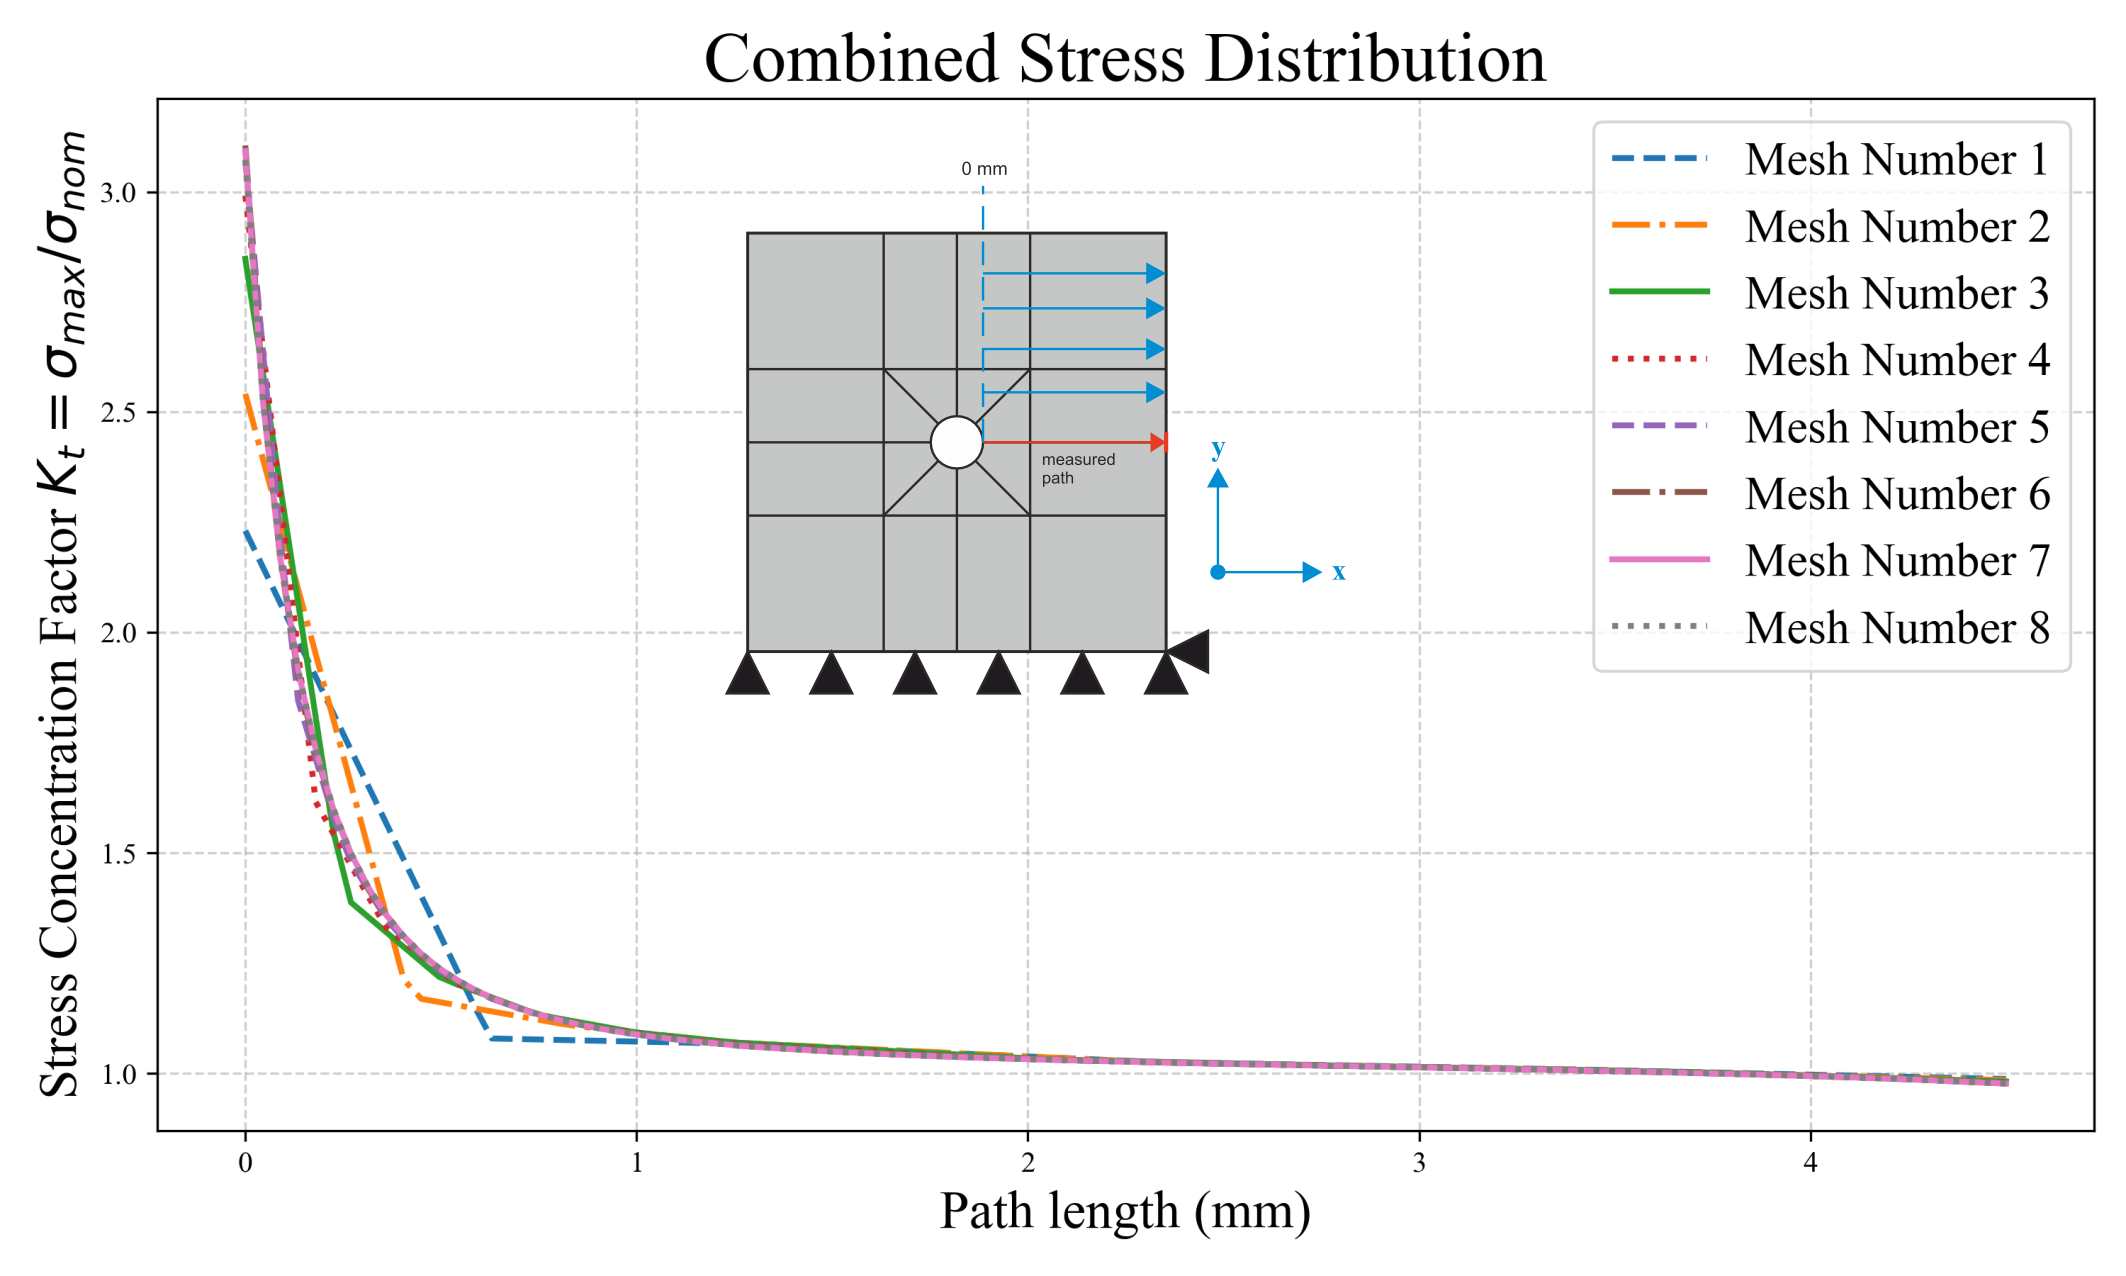
\includegraphics[width=1\textwidth]{images/StressConc.png}
    \caption{Stress distribution along the defined path 
    for all mesh sizes. Each curve represents the relevant stress 
    component for a specific mesh configuration, illustrating the 
    effect of mesh refinement on capturing the stress concentration 
    near the circular hole.}
    \label{fig:CombinedStressDistribution}
\end{figure}

\begin{figure}[H]
    \centering
    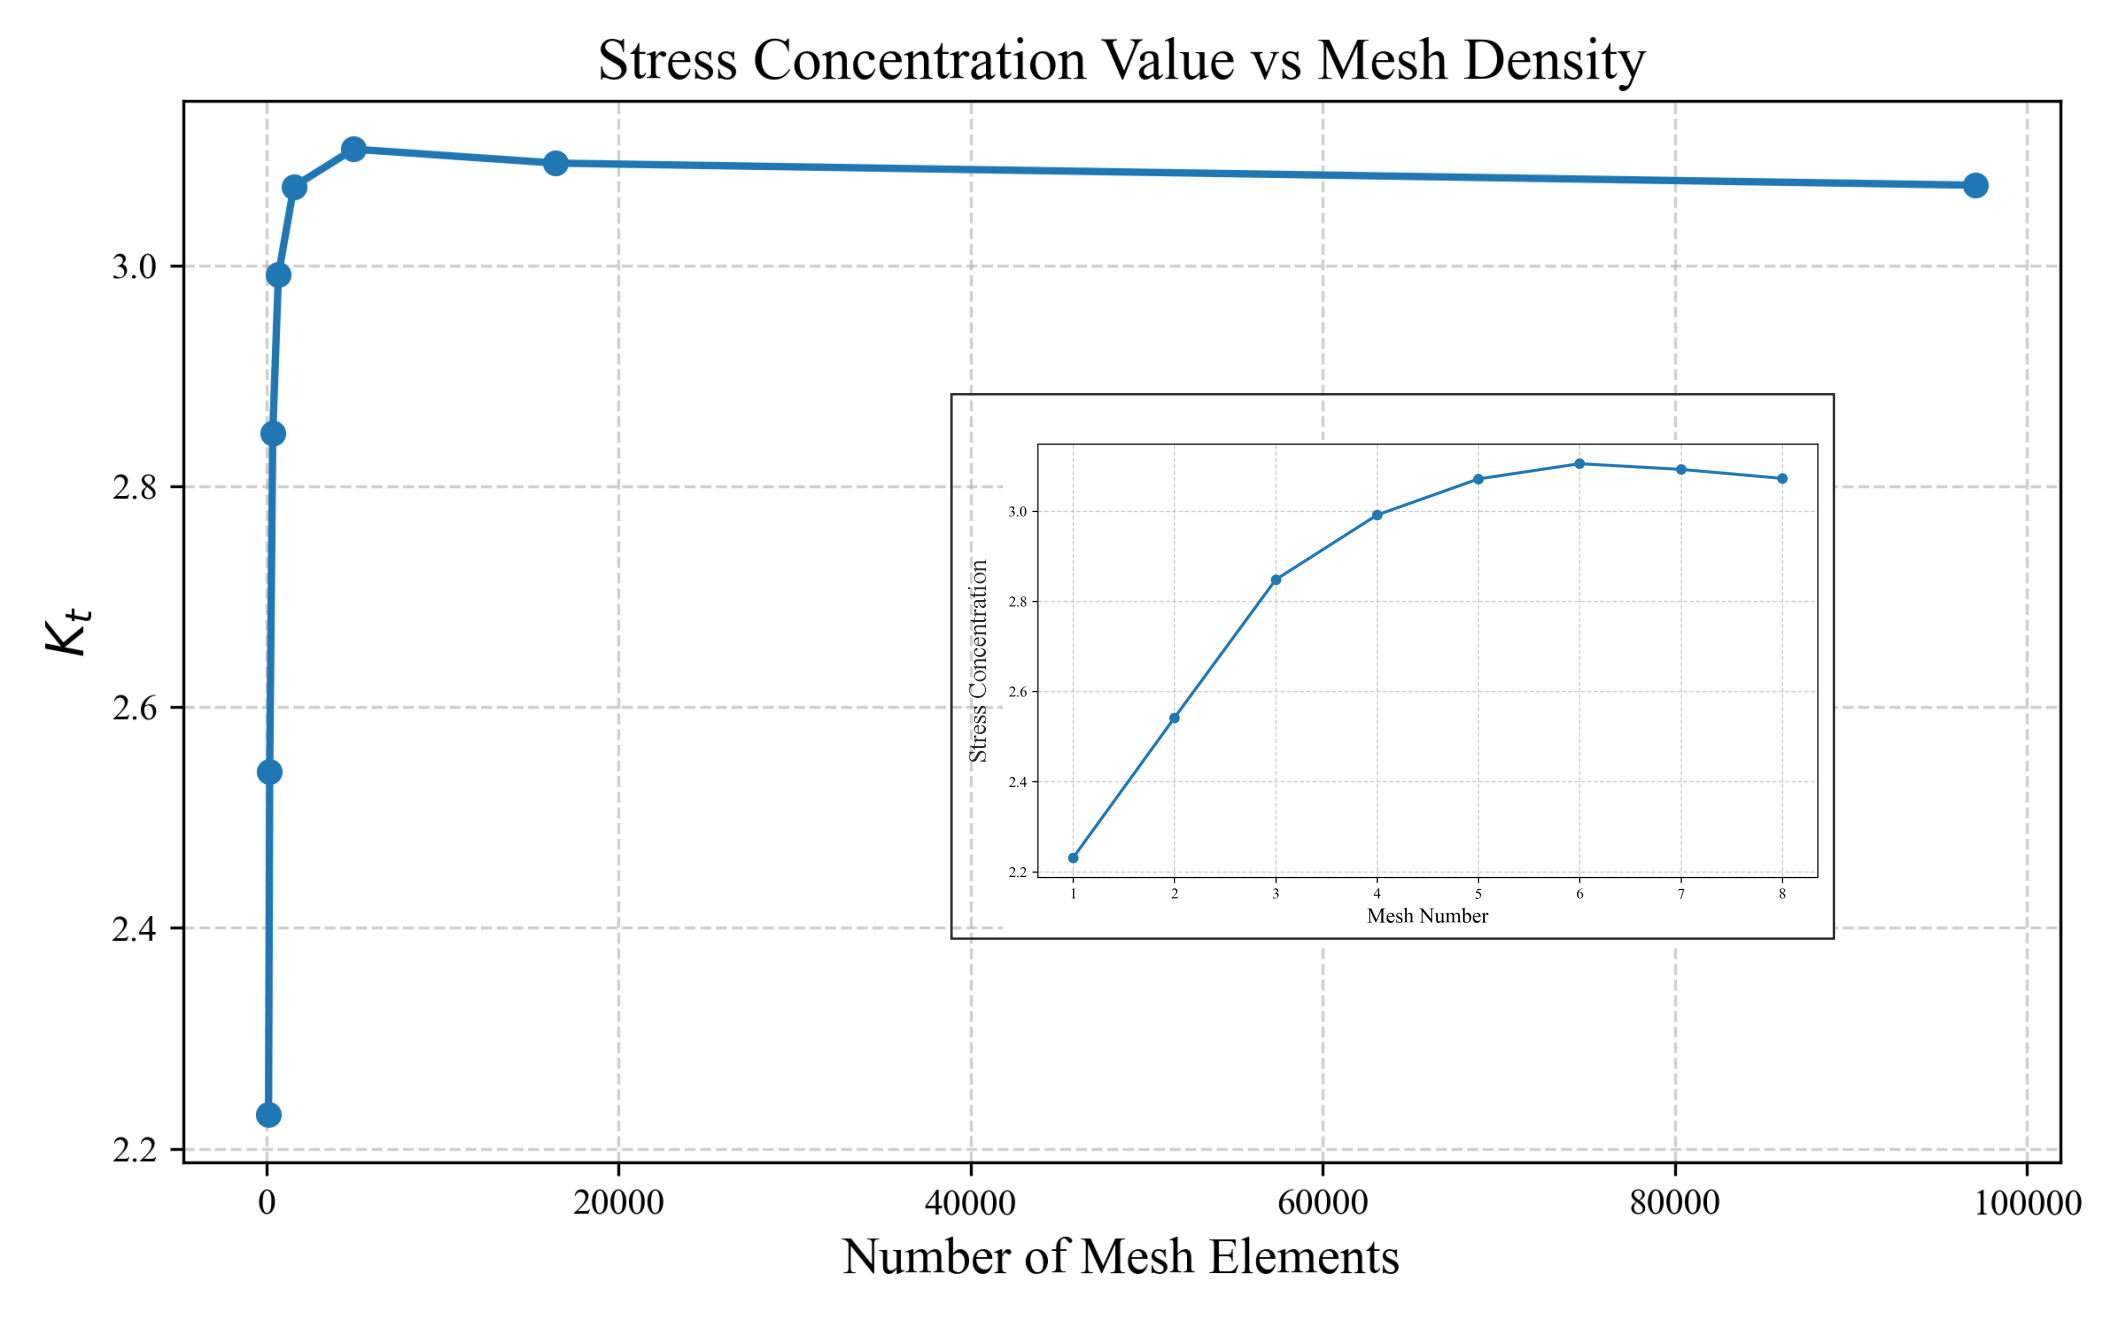
\includegraphics[width=1\textwidth]{images/Kt.png}
    \caption{Stress concentration factor $K_t$ along the defined path 
    for all mesh sizes. Each curve represents the $K_t$ value for a specific mesh configuration, illustrating the 
    effect of mesh refinement on capturing the stress concentration 
    near the circular hole.}
    \label{fig:CombinedStressDistribution}
\end{figure}

\vspace{1em}
\textit{$\dots$ Taking advantage of the symmetry in both the geometry and the boundary conditions, 
propose a simplified model that reduces computational cost and simulation time. 
Create and submit two figures: one showing the mesh of the proposed model, 
and the other displaying contour plot of the relevant stress distribution. 
Compare it to the original model.}


\newpage
\subsection*{Q2: Investigate the effects of isotropic and kinematic hardening on the mechanical behavior of a material}

\vspace{1em}
\textit{$\dots$\textbf{Isotropic Hardening Model:} Set the material parameters for the 
isotropic hardening model, keeping kinematic hardening deactivated. 
Perform a cyclic loading simulation (tension-compression) 
using the amplitude plotted in figure 3. Plot and analyze the stress-strain hysteresis loops.}
\vspace{1em}

\textit{$\dots$\textbf{Kinematic Hardening Model:} Set the material parameters for 
the kinematic hardening model, assuming no isotropic hardening. 
Perform a cyclic loading simulation (tension-compression) using 
the amplitude plotted in figure 3. 
Plot and analyze the stress-strain hysteresis loops.}
\vspace{1em}

\textit{$\dots$Compare the extracted curves from previous questions and discuss the results.}
\vspace{1em}

\textit{$\dots$Simulate the model using combined hardening law parameters in table 2. 
Compare the results with those obtained using isotropic and kinematic hardening parameters. 
Discuss how variations in the combined hardening parameters influence the material behavior.}
\vspace{1em}

\subsection*{Q3: Standard and UMAT subroutine for J2 plasticity}
\vspace{1em}
\textit{$\dots$Read the provided J2 UMAT, then decide to choose plane stress or plane strain condition, add
a screenshot that shows the code lines where this choice is made and where elastic stiffness
and equivalent von mises stress is calculated, and give an explanation based on the lecture.}
\vspace{1em}

\textit{$\dots$Run two simulations with a displacement of 0.5 mm and same material properties: one with
the Abaqus embedded J2 model and one with UMAT. Plot, compare, and discuss the true stress-strain
curve for both cases.}
\vspace{1em}

\textit{$\dots$From the embedded J2 simulation, select four representative time frames that trace the
evolution from the purely elastic status to the onset of localized necking, present for each frame
a contour plot of von Mises stress and equivalent plastic strain. Describe the deformation
process of the plate with a hole.}
\vspace{1em}

\textit{$\dots$From the UMAT simulation, plot the distribution of the relevant stress and plastic strain
components for the final time, indicating the meaning of the different SDVs, showing the
maximum and minimum location, then discussing the results for different regions.}
\vspace{1em}

\section*{Conclusion}
To sum up everything that have been analyzed and gathered in this study, 
here are some several key takeaways from this small case study:
\begin{enumerate}
    \item 
\end{enumerate}

\end{document}

